%-----------------------------------------------------------------
% Requirements and/or Problem Section(s):
% In this section you should describe the problem or system you are addressing in detail. Describe the project requirements and constraints.
%-----------------------------------------------------------------
\subsection{Design Problem}
The problem we are trying to solve is to beat daily fantasy basketball competitions using machine learning. In order to fully understand this problem, it is important to detail daily, top-heavy, fantasy basketball competitions. 
\subsubsection{Competition Choice}
When most people think of fantasy sports, they think of creating a team at the beginning of the sport's season, and following this team through the season. The types of competitions and specific competition rules actually vary greatly, and rather than try to create a system that can handle all of these, we decided to target a specific subset. The competitions we will target must meet the following criteria:
\begin{itemize}
\item Daily competitions
\item Low entry fee (< \$10)
\item High, top-heavy, prize pool
\item Multiple entries allowed
\end{itemize}
Daily competitions are different from the traditionally thought of fantasy season. They occur over a single day, where real basketball games are being played and involve only the games being played that day.
A header for one of these daily competitions on FanDuel.com that meets our other criteria can be seen in figure \ref{fig:comp_header}. This header shows the low entry fee of \$7, the high prize pool of \$100,000, and that multiple entries are allowed. It also shows a list of the real games that are occurring that night.

\begin{figure}[ht]
    \centering
    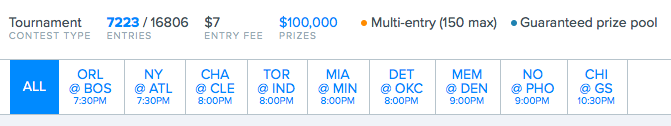
\includegraphics[width=0.75\textwidth]{figures/fantasy_competition_header}
    \caption{Daily NBA fantasy competition header}
    \label{fig:comp_header}
\end{figure}

The third criterion in the list specifies a "top-heavy" prize pool. This was one of the conditions of the Picking Winners paper, and is one of ours, as well. The meaning of top-heavy is that most of the prize-pool winnings go to the top contenders. This is different from a 50-50 contest, where the top 50\% of competitors are given double their entry fee. With top-heavy competitions, "contests give a disproportionately high fraction of the entry fees to the top scoring lineups." \cite{picking_winners}. The entry fees for these competitions are usually less than \$10, and the top placing competitors usually win thousands of dollars. We aim for these types of competitions because we aim to submit many different lineups, each with a high probability of success. The payout structure of a competition with a \$4.44 entry fee and \$400,000 prize-pool can be seen in Figure \ref{fig:comp_payout}. One can see that the difference between first and tenth place is 200 times, whereas the difference between tenth and one-hundredth is only 10 times.

\begin{figure}[ht]
    \centering
    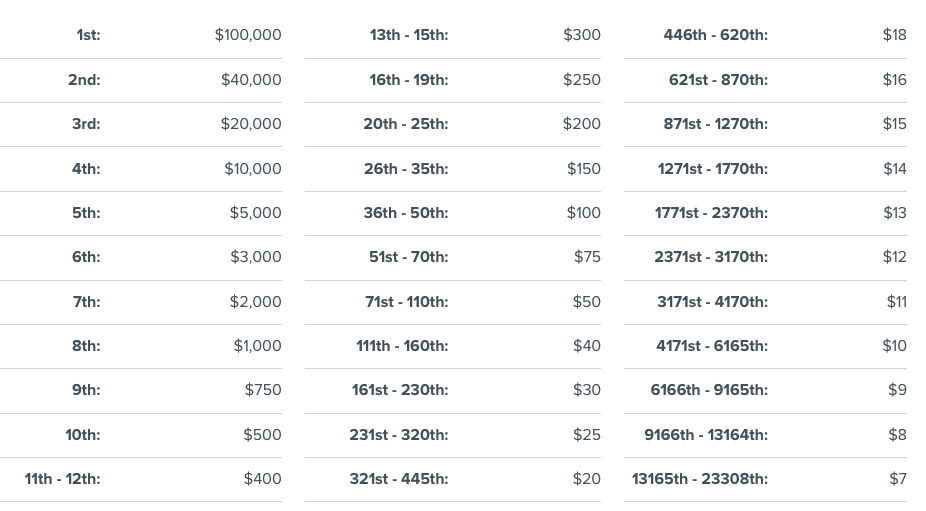
\includegraphics[width=0.75\textwidth]{figures/fantasy_competition_payout}
    \caption{FanDuel daily fantasy competition payout}
    \label{fig:comp_payout}
\end{figure}

The goal is for one or two of our entries to be on the top-heavy side of a competition (not every competition), offsetting the losses of the other entries. Another reason we feel that obtaining a high ranking entry is feasible is because we believe that our system, if successful, will return uncommon lineups that other methods (intuition or optimization) will not return.

\subsubsection{Entries}
After selecting the competition to enter, the participant must create an entry, or lineup. This lineup must comprise players that are playing in the real games on that day. Additionally, the lineup must have a certain amount of specific basketball positions. A common requirement is that the lineup has to have two point guards (PG), two shooting guards (SG), two power forwards (PF), two small forwards (SF), and one center (C). Note that this may not be representative of a real basketball lineup. Figure \ref{fig:comp_lineup} shows the lineup selection interface for FanDuel.com. On the right side, one can see the required positions for a given competition, along with the lineup's budget, in the top right corner. This budget is the amount of money each contender is allowed to spend on their lineup. On the left side, one can see the price of each player, along with their position, and their average fantasy performance for the season, on which the price is dependent.

\begin{figure}[ht]
    \centering
    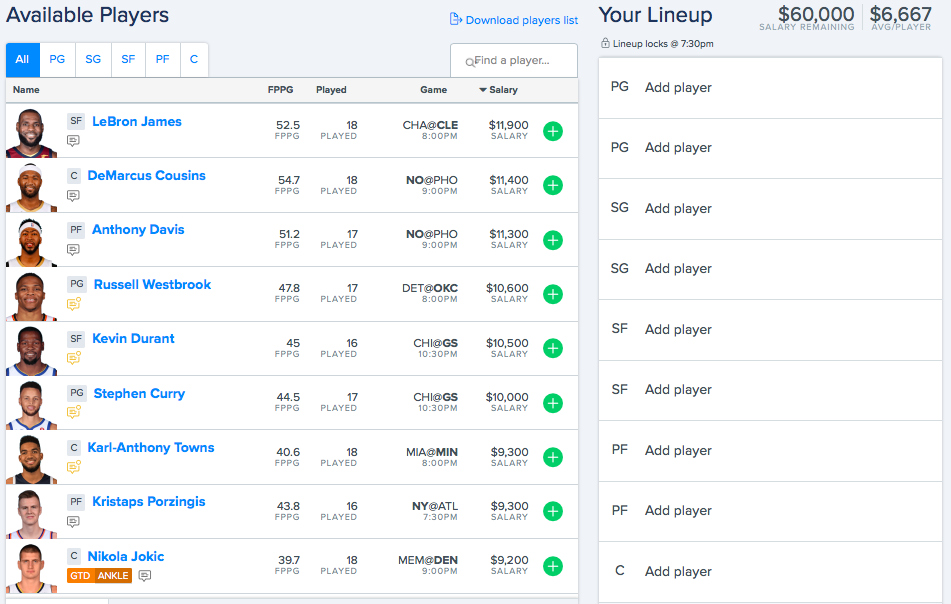
\includegraphics[width=0.75\textwidth]{figures/fantasy_competition_lineup}
    \caption{Fantasy basketball competition lineup}
    \label{fig:comp_lineup}
\end{figure}

\subsubsection{Scoring}
The participant's goal is to have the lineup with the highest score. The score is based on how well their selected players perform in real life, and is based on the amount of free throws, three pointers, field goals, blocks, steals, assists, and turnovers each player gets. A sample scoring system for competitions on FanDuel can be seen in Figure \ref{fig:comp_scoring}.

\begin{figure}[ht]
    \centering
    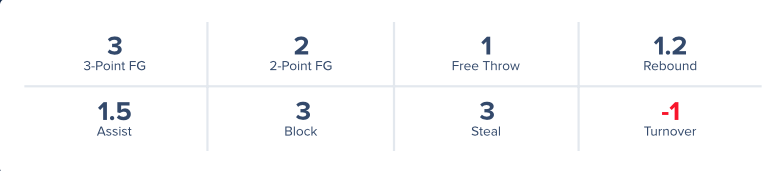
\includegraphics[width=0.75\textwidth]{figures/fantasy_competition_scoring}
    \caption{Fantasy basketball competition scoring}
    \label{fig:comp_scoring}
\end{figure}

\subsection{Requirements and Constraints}
In order to solve the described problem, we had to comply with everything that was mentioned above. However, there are other requirements and constraints which are given below.
\subsubsection{Functional Requirements}
%(e.g. what a product should do)
\begin{itemize}
\item The system should be able to use all previous NBA data
\item The system should be able to output lineups for daily fantasy competitions based on which teams are playing, how much each player costs, and which positions are needed
\item The system should output a projected score for each lineup
\end{itemize}

\subsubsection{Usability Requirements}
%(e.g. security, network, platform, integration, client)
\begin{itemize}
\item The system should use a MySQL database
\item The database should be secure and have personalized credentials for all users
\item The system source code should be version controlled
\end{itemize}

\subsubsection{Technical Requirements}
\begin{itemize}
\item The system should be able to train on the order of magnitude of minutes
\item The system should be modular, allowing for quick and easy changes
\item The system should allow NN parameters and other parameters (data amount) to be changed quickly for testing
\end{itemize}

\subsubsection{Constraints}
\begin{itemize}
\item The system must not require any expensive services
\item The system must be trainable on our personal computers
\item The system must be completed within eight months (two university terms)
\end{itemize}